\documentclass[a4paper, 14pt]{extarticle}

% file's preambule

% Если вы работаете не в XeLaTeX, то сами разбирайтесь =)

% connect packages
%%%%%%%%%%%%%%%%%%%%%%%%%%%%%%%%%%%%%%%%%%%%%%%%%%%%%%%%%%%%%%%%%%%%%%
%\usepackage[T2A]{fontenc}                   %!? закрепляет внутреннюю кодировку LaTeX
%\usepackage[utf8]{inputenc}                 %!  закрепляет кодировку utf8
\usepackage{fontspec}                        % Шрифты
\usepackage{indentfirst}                    %   добавить indent перед первым параграфом
\setlength{\parindent}{1.27cm}
\usepackage{polyglossia}                     % Русский язык
\setdefaultlanguage{russian}
\setmainfont[Ligatures=TeX]{Times New Roman}
\newfontfamily\cyrillicfont{Times New Roman}[Script=Cyrillic]
%\usepackage[english,russian]{babel}         %!  подключает русский и английский
\usepackage{amsmath}                        %!  |
\usepackage{amssymb,textcomp, esvect,esint} %!  |важно для формул 
\usepackage{geometry}                       %!  отступ от граней
\geometry{verbose,a4paper,tmargin=2cm,bmargin=2cm,lmargin=3cm,rmargin=1cm}
\usepackage{amsfonts}                       %!  математические шрифты
\usepackage{amsthm}                         %!  newtheorem и их сквозная нумерация
\usepackage{graphicx}                       %?  графическое изменение текста
\usepackage{soulutf8}% Поддержка переносоустойчивых подчёркиваний и зачёркиваний
\usepackage{enumitem}                       %!  задание макета перечня.
%\usepackage[unicode, pdftex]{hyperref}      %!  оглавление для панели навигации по PDF-документу + гиперссылки
\usepackage{setspace}                       % Межстроковые интервалы
\onehalfspacing
\usepackage{booktabs}                       %!  добавляет книжные линии в таблицы
%\usepackage{hypcap}                         %?  адресация на картинку, а не на подпись к ней
\usepackage{abraces}                        %?  фигурные скобки сверху или снизу текста
\usepackage{caption}                        %-  позволяет корректировать caption 
\DeclareCaptionLabelSeparator{dash}{ - }
\captionsetup[table]{labelformat=simple, labelsep=dash, justification=raggedleft,
singlelinecheck=off}
\captionsetup[figure]{labelformat=simple, labelsep=dash}
\usepackage{multirow}                       %   объединение ячеек в таблицах
\usepackage{longtable}
\usepackage{pifont}                         %!  нужен для крестика
\usepackage{cancel}                         %!  аутентичное перечеркивание текста
\usepackage{ulem}                           %!  перечеркивание текста
\usepackage{tikz}                           %!  высокоуровневые рисунки (кружочек)
\usepackage{titling}                        %-  автоматическое заглавие 
\usepackage{titlesec}  % нормальные заголовки секций
\titleformat{\section}
{\normalfont\large\bfseries\filcenter}{}{1em}{}
\titleformat{\subsection}
  {\normalfont\normalsize\bfseries}{\thesubsection.}{5pt}{}
\titleformat{\subsubsection}
  {\normalfont\normalsize\bfseries}{\thesubsubsection.}{5pt}{}
\titleformat{\paragraph}
  {\normalfont\normalsize\bfseries}{\theparagraph}{5pt}{}

\usepackage{ragged2e} % Для выравнивания текста по ширине
\justifying

%\renewcommand{\thesubsubsection}{\alph{subsubsection}}
\usepackage{blindtext}                      %-  слепой текст
\usepackage{fancyhdr}                       %   добавить верхний и нижний колонтитул
\usepackage{mathptmx}

\usepackage{import}                         %|
\usepackage{xifthen}                        %|
\usepackage{pdfpages}                       %|
%\usepackage{transparent}                    %| вставка ink figures
\usepackage{rotating}
\usepackage{array} % Картиночки в таблицы
%%%%%%%% Алгоритмы
\usepackage{float}
\usepackage{algorithm}
\usepackage{algpseudocode}
%%%%%%%%%%%%%%%

\usepackage{listings} % Для языков программирования 
\usepackage{xcolor}
\lstset {
    language=C++,
    backgroundcolor=\color{black!5}, % set backgroundcolor
    basicstyle=\footnotesize,% basic font setting
}

\usepackage{lmodern}

\colorlet{comment}{green!50!black}
\colorlet{cppcomment}{teal}
\colorlet{symb}{blue!50!black}
\colorlet{number}{violet}

\newcommand*{\textcolorsymb}{\textcolor{symb}}

\definecolor{backcolour}{rgb}{0.95,0.95,0.92}
\definecolor{black_red}{rgb}{0.54, 0, 0}

\lstdefinestyle{cpp}{%
  language=C++,
  columns=flexible,
  basewidth=.5em,  
  tabsize=2,
  basicstyle=\footnotesize,
  backgroundcolor=\color{backcolour},
  showspaces=false,
  showstringspaces=false,
  commentstyle={\itshape\color{comment}\let\textcolorsymb\relax},
  keywordstyle=\bfseries\color{black_red},
  morecomment={[l][\itshape\color{cppcomment}\let\textcolorsymb\relax]//},
  literate=%
    {\{}{\textcolorsymb{\{}}1
    {\}}{\textcolorsymb{\}}}1
    {(}{\textcolorsymb{(}}1
    {)}{\textcolorsymb{)}}1
    {;}{\textcolorsymb{;}}1
    {=}{\textcolorsymb{=}}1
    {<}{\textcolorsymb{<}}1
    {>}{\textcolorsymb{>}}1
    {!}{\textcolorsymb{!}}1
    {\&}{\textcolorsymb{\&}}1 
    {|}{\textcolorsymb{|}}1
    {?}{\textcolorsymb{?}}1
    {:}{\textcolorsymb{:}}1
    {+}{\textcolorsymb{+}}1
    {-}{\textcolorsymb{-}}1
    {,}{\textcolorsymb{,}}1
    {\%}{\textcolorsymb{\%}}1
    {\^}{\textcolorsymb{\textasciicircum}}1
    {~}{\textcolorsymb{\textasciitilde}}1
    %% {/}{\textcolorsymb{/}}1
    %% {*}{\textcolorsymb{*}}1
    % 2 (optionally)
    {==}{\textcolorsymb{==}}2
    {>=}{\textcolorsymb{=>}}2
    {<=}{\textcolorsymb{<=}}2
    {!=}{\textcolorsymb{!=}}2
    {+=}{\textcolorsymb{+=}}2
    {-=}{\textcolorsymb{-=}}2
    {*=}{\textcolorsymb{*=}}2
    {/=}{\textcolorsymb{/=}}2
    {\%=}{\textcolorsymb{\%=}}2
    {\&\&}{\textcolorsymb{\&\&}}2
    {||}{\textcolorsymb{||}}2
    {++}{\textcolorsymb{++}}2
    {--}{\textcolorsymb{--}}2
    {>>}{\textcolorsymb{>\kern0pt>}}2
    {<<}{\textcolorsymb{<\kern0pt<}}2
    {::}{\textcolorsymb{::}}2
    % 3 (optionally)
    {>>=}{\textcolorsymb{>\kern0pt>=}}3
    {<<=}{\textcolorsymb{<\kern0pt<=}}3
    % Remove byte order mark
    {^^ef^^bb^^bf}{}0
}
\lstnewenvironment{cpp}{\lstset{style=cpp}}{}
\lstset{style=cpp}
  


%%%%%%%%%%%%%%%%%%%%%%%%%%%%%%%%%%%%%%%%%%%%%%%%%%%%%%%%%%%%%%%%%%%%%%


%%%%%%%%%%%%%%%%%% ВСТАВКА РИСУНКО ИЗ INKSCAPE %%%%%%%%%%%%%%%%%%%%%%%
\newcommand{\incfig}[1]{%
    \def\svgwidth{\columnwidth}
    \import{./figures/}{#1.pdf_tex}
}

%%%%%%%%%%%%%%%%%%%%%%%%%%%%%%%%%%%%%%%%%%%%%%%%%%%%%%%%%%%%%%%%%%%%%%


\newenvironment{itemize*}
{
    \begin{itemize}
        \setlength{\itemsep}{1pt}
        \setlength{\parskip}{1pt}}
    {\end{itemize}
}

\newenvironment{enumerate*}
{
    \begin{enumerate}
        \setlength{\itemsep}{1pt}
        \setlength{\parskip}{1pt}}
    {\end{enumerate}
}

%%%%%%%%%%%%%%%%%%%%%%%%%%%%%%%%%%%%%%%%%%%%%%%%%%%%%%%%%%%%%%%%%%%%%%


\begin{document}

\includepdf{titul_seventh}
\newpage
\tableofcontents
\newpage
\section{Главное задание}
\subsection{Постановка задачи}
Разработать многомодульную программу, которая демонстрирует
выполнение всех операций, определенных вариантом, над линейным
двунаправленным динамическим списком и функции для работы с этой структурой:

\subsection{Определение операций над списком}
\paragraph{Определение структуры узла двунаправленного списка}
Согласно варианту No9 в качестве информационной части узла списка
используются поля: марка автомобиля, страна изготовитель,
год выпуска.
\paragraph{Описание обязательных операций над списком}

\textit{Обязательные:}
\begin{enumerate}
  \item Вывод списка в двух направлениях.
  \item Поиск узла с заданным значением.

    \textit{Функции дополнительного задания варианта:}
  \item Вставка узла по автомобилю в списке своего модельного ряда
    перед узлом, год выпуска которого меньше.
  \item Формирование нового списка с узлом вида ("модельный" узел): марка автомобиля
    и указатель на начало модельного ряда данной марки в исходном списке.
  \item Удаление информации обо всех автомобилях заданной марки.
\end{enumerate}

\newpage
\paragraph{Алгоритмы операций над списком}
\begin{figure}[htpb]
  \centering
  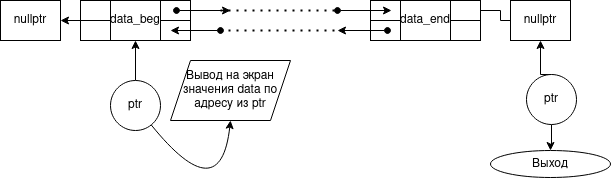
\includegraphics[width=0.8\textwidth]{pictures/print_list.png}
  \caption{Алгоритм вывода списка как в прямом, так и обратном направлениях}
  \label{fig:print_list}
\end{figure}
\begin{figure}[htpb]
  \centering
  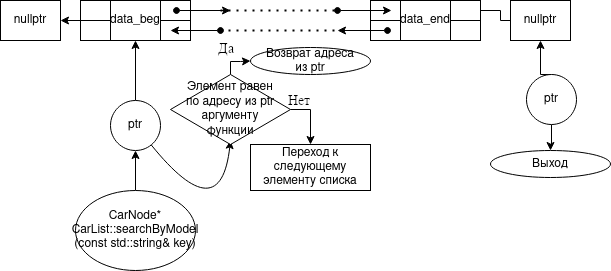
\includegraphics[width=0.8\textwidth]{pictures/search_model_ok.png}
  \caption{Алгоритм поиска первого элемента с заданным названием модели}
  \label{fig:search_model}
\end{figure}
\begin{figure}[htpb]
  \centering
  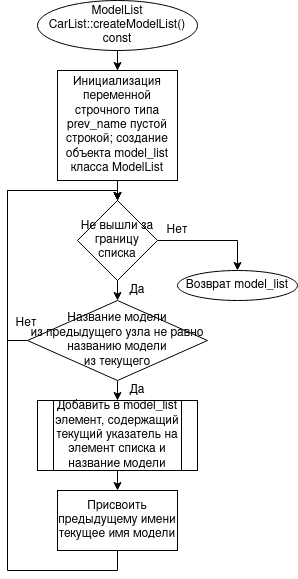
\includegraphics[width=0.6\textwidth]{pictures/createList.png}
  \caption{Алгоритм создания списка с "модельными" узлами}
  \label{fig:create_list}
\end{figure}
\begin{figure}[htpb]
  \centering
  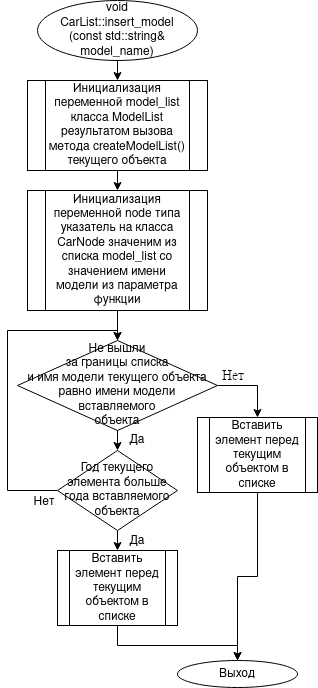
\includegraphics[width=0.4\textwidth]{pictures/insert_model_fix.png}
  \caption{Алгоритм вставки элемента перед той же моделью с меньшим годом}
  \label{fig:create_list}
\end{figure}
\begin{figure}[htpb]
  \centering
  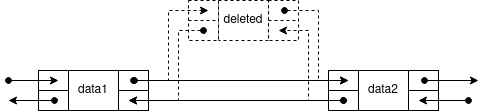
\includegraphics[width=0.8\textwidth]{pictures/delete_row.png}
  \caption{Алгоритм удаления одного узла (требуется в следующем алгоритме)}
  \label{fig:create_list}
\end{figure}
\begin{figure}[htpb]
  \centering
  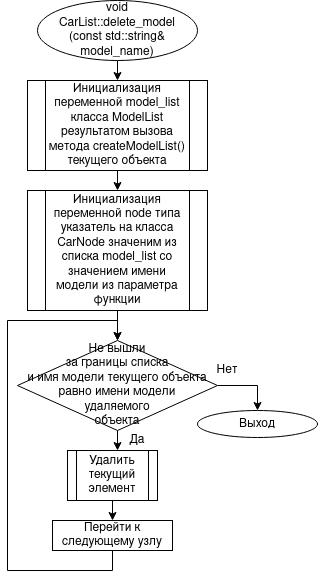
\includegraphics[width=0.6\textwidth]{pictures/delete_model.png}
  \caption{Алгоритм удаления всех элементов с заданным названием модели}
  \label{fig:create_list}
\end{figure}
\newpage
\subsection{Код программы}
Реализация на C++:

\textit{Код файла car\_list.h}
\lstinputlisting{code/car_list.h}

\textit{Код файла car\_list.cpp}
\lstinputlisting{code/car_list.cpp}

\textit{Код файла linked\_list.cpp}
\lstinputlisting{code/linked_list.cpp}
\newpage
\subsection{Результаты тестирования}
\begin{figure}[htpb]
  \centering
  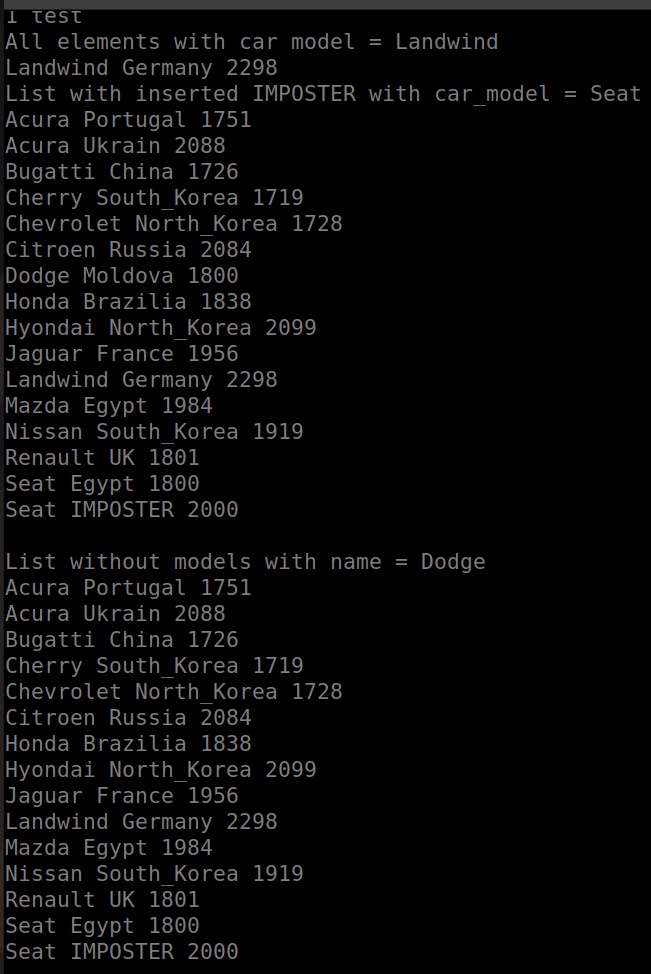
\includegraphics[width=0.7\textwidth]{pictures/first_test.png}
  \caption{Результаты тестирования программы 1 тест}
  \label{fig:test1}
\end{figure}
\newpage
\begin{figure}[htpb]
  \centering
  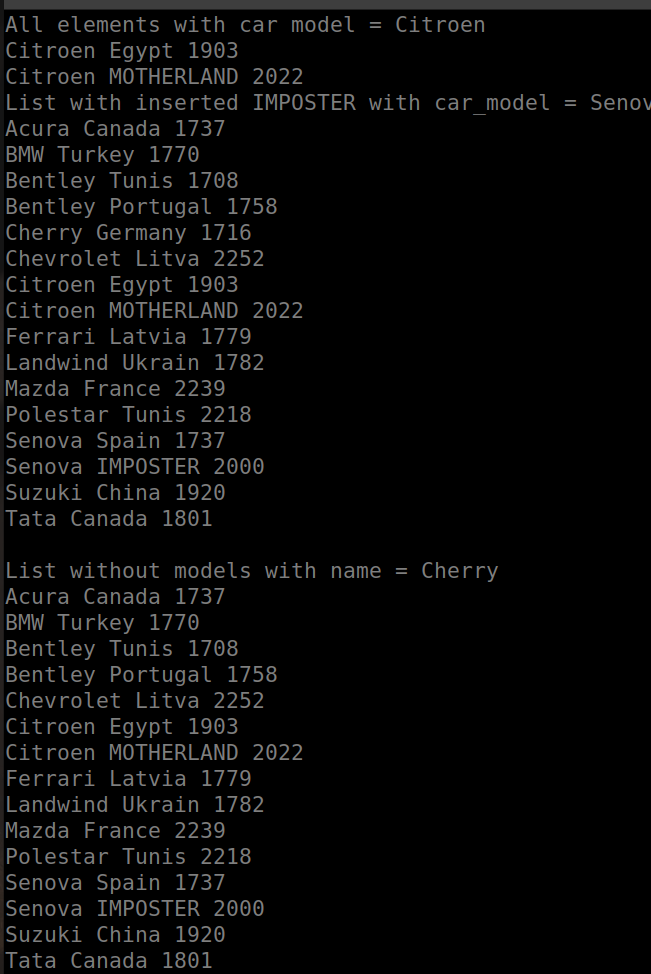
\includegraphics[width=0.7\textwidth]{pictures/second_test.png}
  \caption{Результаты тестирования программы 2 тест}
  \label{fig:test2}
\end{figure}
\subsection{Сложность первой дополнительной операции (вставка в список)}
\begin{enumerate}
  \item На линейном динамическом списке $T(n)=\Theta(n)$ т.к. для вставки
    необходимо получить нужный адрес элемента, что занимает  $\Theta(n)$ времени
    в среднем случае. 
  \item На одномерном массиве также $T(n)=\Theta(n)$ т.к. для вставки все равно
    необходимо получить адрес элемента, перед которым необходимо вставлять,
    что занимает  $\Theta(n)$ в среднем случае.
\end{enumerate}
\newpage
\section*{Выводы}
\addcontentsline{toc}{section}{Выводы}
В ходе выполнения работы была реализована структура
«двунаправленный список», поддерживающий следующие обязательные операции: вывод
хранящихся значений узлов списка в прямом и обратном порядках; поиск первого
элемента в списке по заданной модели; вставка нового узла перед узлом,
год выпуска которого меньше; создание списка с "модельными" узлами;
удаление всех элементов с заданным названием модели. Также в ходе
выполнения работы были усвоены основы работы с двунаправленными списками.
Тестирование подтвердило правильность работы методов.
\section*{Список информационных источников}
\addcontentsline{toc}{section}{Список информационных источников}
\begin{enumerate}[leftmargin=*]
  \item Thomas H. Cormen, Clifford Stein и другие: Introduction to Algorithms, 3rd Edition.
    Сентябрь 2009. The MIT Press.
  \item N. Wirth: Algorithms and Data Structures. Август 2004.
    \\ https://people.inf.ethz.ch/wirth/AD.pdf.
  \item Linked list~//~Wikipedia \\~
    [Электронный ресурс]. URL:
    \\ https://en.wikipedia.org/wiki/Linked\_list
    (Дата обращения: 02.05.2021)
   \item Курс Algorithms, part 2 // Coursera [Электронный ресурс]. URL:
     \\ https://www.coursera.org/learn/algorithms-part2
     (Дата обращения: 02.05.2021)
\end{enumerate}
\end{document}
